\documentclass[11pt, uplatex, dvipdfmx]{jsarticle}
\usepackage{amsmath,amsfonts, bm, braket, setspace, emathEy, enumitem, graphicx}

\newcommand*{\ds}{\displaystyle}
\renewcommand*{\dlim}{\lim\limits} %emathEyを使わないなら\newcommand
\renewcommand*{\vec}[1]{\overrightarrow{\textrm{#1}}}

\resettagform


\pagestyle{plain}



\title{\Huge 線形代数 問題集}


\begin{document}

\maketitle
\thispagestyle{empty}

\newpage

\section{行列の演算}\label{sec:matrix}

\begin{enumerate}[label=\ref{sec:matrix}.\arabic*]
  \setlength{\itemsep}{1zh}
  
\item 次の行列 $A$ に対し,$A^n$ を求めよう.ただし,$n$ は自然数とする.

  \vspace{1ex}
  
  \begin{edaenumerate}<retusuu=3>[(1)]
  \item $A= \left[
      \begin{array}{rr}
        2 & 1\\
        0 & 2
      \end{array}
    \right]$

  \item $A=\left[
      \begin{array}{rrr}
        2 & 1 & 0\\
        0 & 2 & 0\\
        0 & 0 & 3
      \end{array}
    \right]$
    
  \item $A=\left[
      \begin{array}{rrr}
        2 & 1 & 0\\
        0 & 2 & 1\\
        0 & 0 & 2
      \end{array}
    \right]$
  \end{edaenumerate}\vspace{-2zh}

\item $B=\left[
    \begin{array}{rr}
      2 & 1\\
      0 & 2
    \end{array}
  \right], \; P=\left[
    \begin{array}{rr}
      3 & 4\\
      2 & 3
    \end{array}
  \right]$ とする.

  \vspace{1zh}
  
  \begin{enumerate}[label=(\arabic*)]
    \setlength{\itemsep}{1ex}
    
  \item $P^{-1}AP=B$ となる行列 $A$ を求めよう.

  \item 自然数 $n$ に対し,$A^n$ を求めよう.
  \end{enumerate}

\item $A=\left[
    \begin{array}{rr}
      -2 & 2\\
      5 & -3
    \end{array}
  \right]$ とする.

  \vspace{1zh}

  \begin{enumerate}[label=(\arabic*)]
    \setlength{\itemsep}{1ex}
    
  \item $A^2+5A-4E_2$ を計算しよう.

  \item (1) の結果を活用して $A^5$ を効率良く計算しよう.
  \end{enumerate}
  
\item 下図のような $5$ 個の空港 $1, 2, 3, 4 ,5$ を結ぶ航空路線がある.
  空港 $i$ から空港 $j$ への直通路線があるとき $a_{ij}=1$ とし,そうで
  ないとき $a_{ij}=0$ とする.ただし,$a_{ii}=0$ とする.
  \begin{figure}[h]
    \centering
    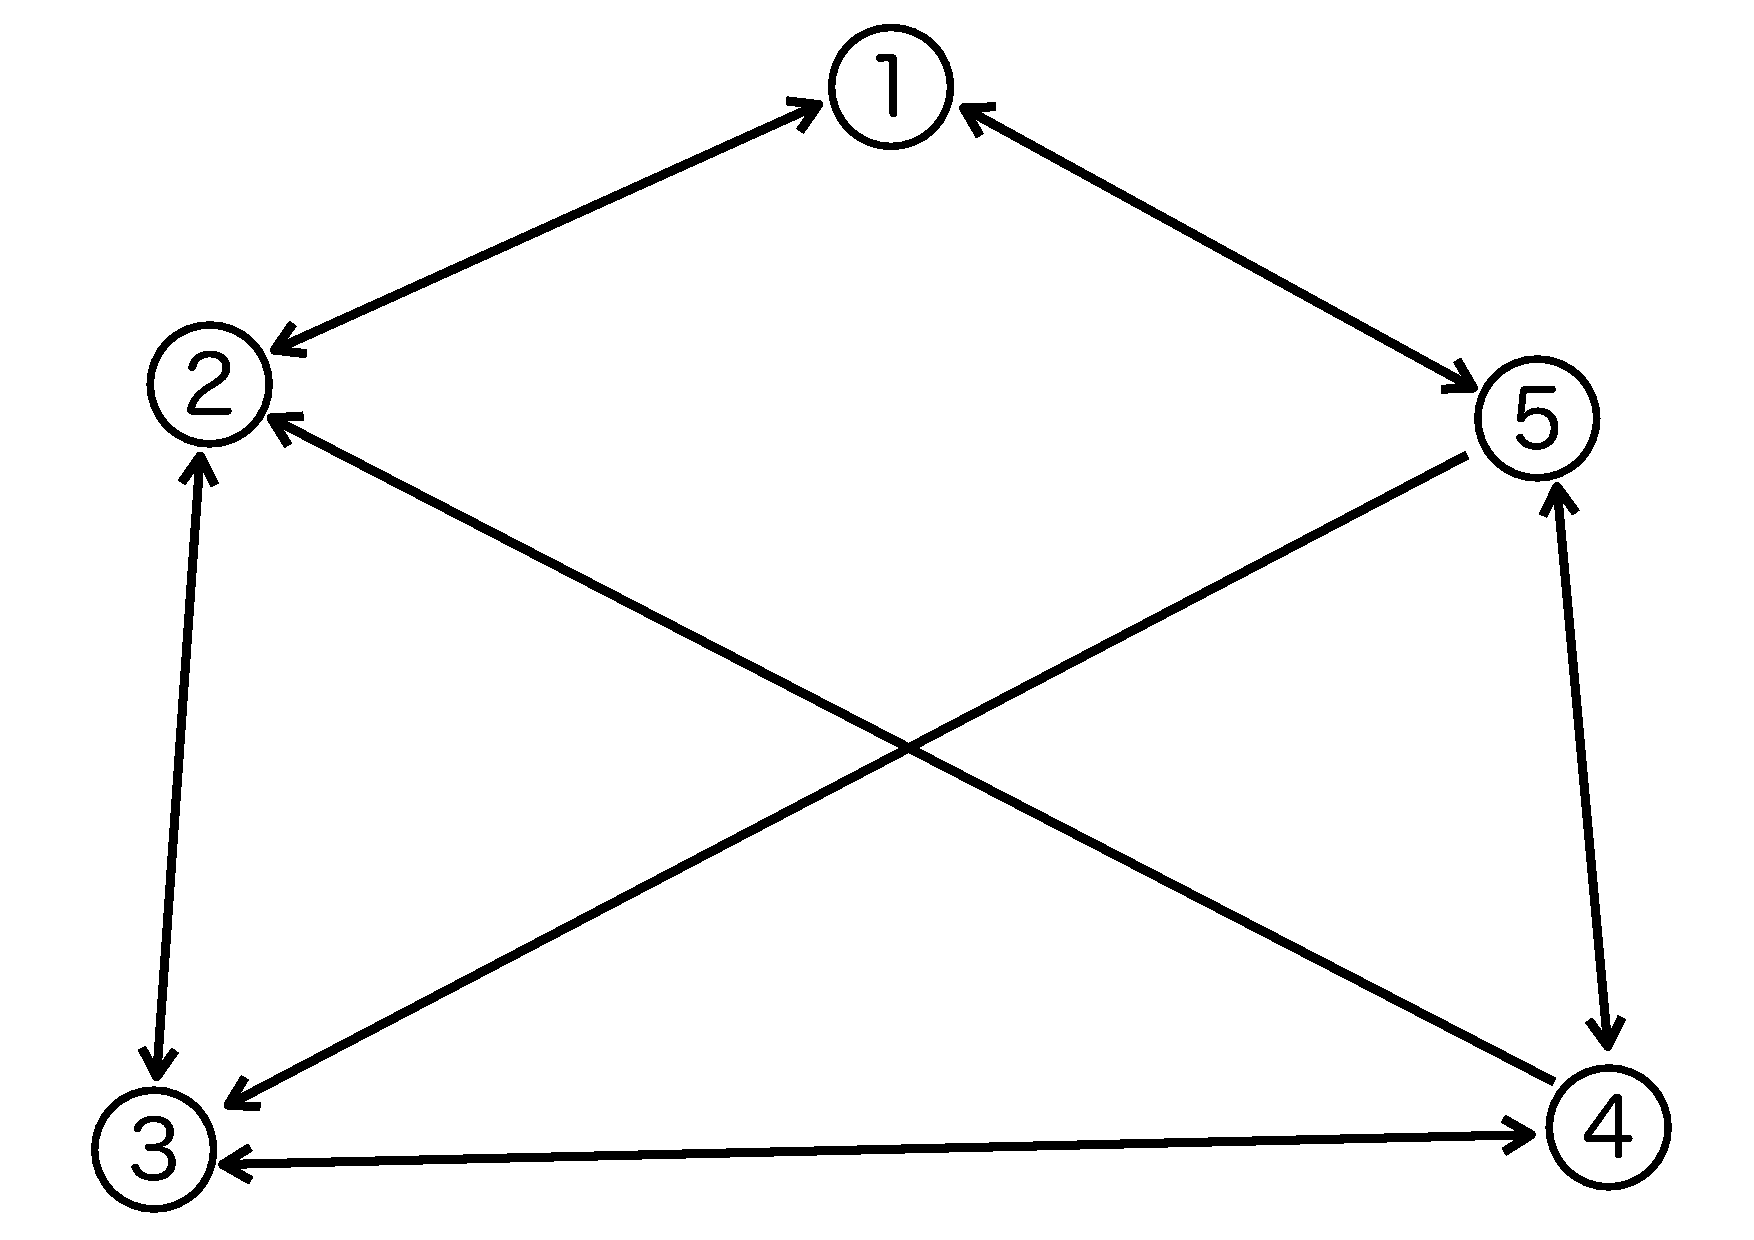
\includegraphics[width=6cm]{./pictures/routes.pdf}
  \end{figure}

  \begin{enumerate}[label=(\arabic*)]
    \setlength{\itemsep}{1ex}
    
  \item $a_{ij}$ を $(i,j)$ 成分とする $5$ 次正方行列 $A=\left[ a_{ij}\right]$ を具体的に書いてみよう.

  \item $A^2, A^3, A^4$ を計算しよう.

  \item $A^2$ の $(i,j)$ 成分は
    $a_{i1} a_{1j} + a_{i2}a_{2j} + a_{i3}a_{3j} + a_{i4}a_{4j} +
    a_{i5}a_{5j}$ であることから,この値が何を意味するか考えよう.

  \item 自然数 $n$ に対して $A^n$ の $(i,j)$ 成分が何を意味するか考えよう.

  \item 路線 $4 \to 2 \to 1 \to 5 \to 3$ のように,空港 $4$ から出発し
    て $4$ 回の移動($3$ 回の乗り継ぎ)で空港 $3$ に到着する路線の個数
    を求めよう.
  \end{enumerate}


\end{enumerate}

\section{連立1次方程式}\label{sec:system}

\begin{enumerate}[label=\ref{sec:system}.\arabic*]
  \setlength{\itemsep}{1zh}


\item 以下を満たす $3$ 次関
  数 $f(x)=a_0 + a_1 x + a_2 x^2 + a_3 x^3$ の係数を決定しよう.
  \[
    f(1)=1, \quad f(2)=2, \quad f'(1)=2, \quad f'(2)=3
  \]
  
\item 行基本変形と基本行列に関する問題を作りたい
  
\item $\bm{a}_1 = \left[
    \begin{array}{r}
      2\\
      2\\
      -1
    \end{array}
  \right], \; \bm{a}_2=\left[
    \begin{array}{r}
      1\\
      3\\
      -4
    \end{array}
  \right], \; \bm{b} = \left[
    \begin{array}{r}
      5\\
      2\\
      5
    \end{array}
  \right], \; A=\left[
    \begin{array}{cc}
      \bm{a}_1 & \bm{a}_2
    \end{array}
  \right]$ とする.
      
  \vspace{1zh}

  \begin{enumerate}[label=(\arabic*)]
    \setlength{\itemsep}{1ex}
    
  \item 連立1次方程式 $A\bm{x} = \bm{b}$ を解こう.

  \item 連立 $1$ 次方程式 ${}^{t}A A\bm{x} = {}^{t}A \bm{b}$ を解こう.

  \item (2) で求めた解 $\bm{x}$ に対して,空間ベクトルの内
    積 $(A\bm{x}) \cdot (A\bm{x} -\bm{b})$ を計算しよう.

  \item 空間ベクトル $A\bm{x}-\bm{b}$ の大きさの $2$ 乗 $|A\bm{x} - \bm{b}|^2$ が最小とな
    る $\bm{x}$ を求めよう.
  \end{enumerate}
    
\end{enumerate}

\newpage

\section{行列式}\label{sec:determinant}

\begin{enumerate}[label=\ref{sec:determinant}.\arabic*]
  \setlength{\itemsep}{1zh}
  
\item 

  \begin{enumerate}[label=(\arabic*)]
    \setlength{\itemsep}{1ex}
    
  \item O を原点とする $xy$ 平面上に $3$ 点 A$(a,c)$, B$(b,d)$,
    C$(a+b, c+d)$ があり,$\vec{OA}$ と $\vec{OB}$ は平行でないとする.
    平行四辺形 OACB と三角形 OAB の面積を求めよう.

  \item $2$ 次正方行列 $\left[
      \begin{array}{cc}
        a & b\\
        c & d
      \end{array}
    \right]$ の行列式を計算しよう.

  \item $5$ 点 P$(4,4)$, Q$(-2,6)$, R$(-5,1)$, S$(-3,-3)$, T$(5,-3)$ を
    頂点とする五角形 PQRST の面積を求めよう.
  \end{enumerate}

\item 空間ベクトル $\bm{a} = {}^{t}\left[
    \begin{array}{ccc}
      a_1 & a_2 & a_3
    \end{array}
  \right], \; \bm{b}=  {}^{t}\left[
    \begin{array}{ccc}
      b_1 & b_2 & b_3
    \end{array}
  \right]$ に対して
  \[
    \bm{a} \times \bm{b} = \left|
      \begin{array}{cc}
        a_2 & b_2\\
        a_3 & b_3
      \end{array}
    \right| \bm{e}_1 -\left|
      \begin{array}{cc}
        a_1 & b_1\\
        a_3 & b_3
      \end{array}
    \right|\bm{e}_2 + \left|
      \begin{array}{cc}
        a_1 & b_1\\
        a_2 & b_2
      \end{array}
    \right| \bm{e}_3 = \left|
      \begin{array}{ccc}
        a_1 & b_1 & \bm{e}_1\\
        a_2 & b_2 & \bm{e}_2\\
        a_3 & b_3 & \bm{e}_3
      \end{array}
    \right|
  \]
  を $\bm{a}$ と $\bm{b}$ の外積という.($\bm{e}_1, \bm{e}_2,
  \bm{e}_3$ を形式的に数のように扱って行列式を計算する)

  \vspace{1zh}

  \begin{enumerate}[label=(\arabic*)]
    \setlength{\itemsep}{1ex}
    
  \item 内積 $\bm{a} \cdot (\bm{a} \times \bm{b})$ と $\bm{b}\cdot ( \bm{a} \times \bm{b})$ を計算しよう.

  \item 空間ベクトル $\bm{a} \times \bm{b}$ の大きさ $|\bm{a} \times \bm{b}|$ を求めよう.

  \item 空間ベクトル $\bm{a}$ と $\bm{b}$ が張る平行四辺形の面積を求めよう.
    
  \end{enumerate}

\item ${}^{t}\bm{a}=\left[
    \begin{array}{ccc}
      a_1 & a_2 & a_3
    \end{array}
  \right], \; {}^{t}\bm{b}=\left[
    \begin{array}{ccc}
      b_1 & b_2 & b_3
    \end{array}
  \right], \; {}^{t}\bm{c} = \left[
    \begin{array}{ccc}
      c_1 & c_2 & c_3
    \end{array}
  \right]$ とする.

  \vspace{1zh}
  
  \begin{enumerate}[label=(\arabic*)]
    \setlength{\itemsep}{1ex}
    
  \item 空間ベクトル $\bm{a}$ と $\bm{b}$ と $\bm{a} \times \bm{b}$ が
    張る平行六面体の体積を求めよう.
    
  \item 空間ベクトル $\bm{a}$ と $\bm{b}$ と $\bm{c}$ が張る平行六面体の体積を求めよう.

  \item 空間ベクトルの内積 $(\bm{a} \times \bm{b}) \cdot \bm{c}$ を計算しよう.

  \item $3$ 次正方行列 $A=\left[
      \begin{array}{ccc}
        \bm{a} & \bm{b} & \bm{c}
      \end{array}
    \right]$ の行列式を計算しよう.
      
  \end{enumerate}
  
\item 四面体の体積とか表面積を計算したい
\end{enumerate}

\end{document}
